\documentclass[10pt]{article}
\usepackage{icmlko}

\icmlmeta{IP 파운데이션 월드모델}{258}{자리가 좁아진다}{도메인 전용 축은 공짜가 아니다 --- 웹툰은 제 축으로 $+$0.021 얻고 남의 축으로 $-$0.028 잃는다}

\begin{document}

\twocolumn[
\icmlheader

\begin{abstract}
노트 255 · 257이 웹툰과 애니에 태그 내용 축을 놓아 판을 0.4569에서 0.4687로
올렸다. 네 번째로 모바일(몫 16.9\%)을 쟀다. \texttt{genres} $+$ \texttt{langs}
로 토큰 46종을 만들면 \textbf{성분 둘이 검사를 통과한다} --- 연도 통제
$-$0.239(겹침 0.196) · $+$0.319(겹침 0.343), 조각 부호 둘 다 5/5. 성분 0 은
연도 통제 $+$0.254 로 더 센데 겹침이 \textbf{0.814}(\texttt{target\_breadth})
라 노트 256의 흐린 사본으로 걸러졌다 --- 새 검사가 처음으로 실전에서 일을
했다. \textbf{그런데 판이 안 움직인다}: 모바일이 $+$0.0375($t{=}2.12$) 오르고
\textbf{웹툰이 $-$0.0205($t{=}-6.27$)} 내려 판은 $-$0.0009($t{=}-0.26$)다.
상쇄 13배. 안 넣는다. 그리고 웹툰의 그 손해가 처음이 아니었다 --- 노트 257에서
애니 축이 들어올 때도 $-$0.0075 를 냈다. 넷을 쌓아 재 보니 무늬가 뚜렷하다:
웹툰 $\rho$ 가 0.3805 $\to$ \textbf{0.4018}(제 축) $\to$ 0.3943(애니 들어옴)
$\to$ \textbf{0.3737}(모바일 들어옴)이다. \textbf{제 축으로 $+$0.0213 얻고
남의 축으로 $-$0.0281 잃어, 시작보다 아래로 내려간다.} 판은 그 사이 계속
올랐다(0.4569 $\to$ 0.4687). 노트 250이 ``전용 이름은 가법''이라 했고 판
수준에서는 맞다(교차항 $-$0.0016). \textbf{도메인 수준에서는 아니다} ---
가법성이 도메인 간 이전을 덮고 있었다. 노트 247이 ``판은 자리바꿈에 눈이
없다''고 한 것의 세 번째 얼굴이고, 이번엔 그 자리바꿈이 \emph{우리가 축을
더할수록} 커진다.
\end{abstract}
]

\section{새 검사가 처음으로 일했다}

모바일 레코드에는 \texttt{genres}(36종)와 \texttt{langs}(66종)가 있다. 토큰
46종으로 같은 SVD 를 돌렸다.

\begin{center}\small
\begin{tabular}{lrrrl}
\hline
성분 & 연도 통제 & 조각 & 겹침 & 상대 \\
\hline
0 & $+$0.254 & 5/5 & \textbf{0.814} & \texttt{target\_breadth} \\
1 & $-$0.096 & 5/5 & 0.175 & \\
\textbf{2} & $-$0.239 & 5/5 & 0.196 & \texttt{entry\_friction} \\
\textbf{3} & $+$0.319 & 5/5 & 0.343 & \texttt{wiki\_volatility} \\
\hline
\end{tabular}
\end{center}

성분 0 이 눈에 띈다 --- 연도 통제 $+$0.254 에 조각 5/5 로, 노트 239의 옛
검사 둘만 보면 \textbf{제일 좋은 후보}다. 그런데 겹침이 0.814 다. 노트 256이
붙인 세 번째 검사가 아니었으면 이것을 골랐을 것이고, 노트 256의 세계애니
성분(겹침 0.621, 판 $-$0.0037)보다 더 나빴을 것이다. \textbf{검사가 처음으로
실전에서 후보를 걸렀다.}

\section{판이 안 움직인다}

통과한 둘(2 · 3)을 넣었다.

\begin{center}\small
\begin{tabular}{lrr}
\hline
 & 21축 & 23축 \\
\hline
F21 능형 & 0.4489 & 0.4529 ($+$0.0039) \\
F18 나무 & 0.4571 & 0.4562 ($-$0.0007) \\
\textbf{F23 판} & \textbf{0.4687} & \textbf{0.4678} ($-$0.0009) \\
\hline
\end{tabular}
\end{center}

도메인별로 보면 왜인지 바로 나온다.

\begin{center}\small
\begin{tabular}{lrrr}
\hline
도메인 & 차 & 짝 SE & $t$ \\
\hline
\textbf{모바일} & $+$0.0375 & 0.0177 & \textbf{2.12} \\
\textbf{웹툰} & $\mathbf{-0.0205}$ & 0.0033 & $\mathbf{-6.27}$ \\
아이돌 & $-$0.0687 & 0.0537 & $-$1.28 \\
펀딩 & $-$0.0172 & 0.0128 & $-$1.34 \\
\hline
\end{tabular}
\end{center}

모바일이 얻는 만큼 웹툰이 낸다. \texttt{rank.spread} 로 진짜 총량이 0.0119
인데 순이 $-$0.0009 --- \textbf{상쇄 13배}다. 노트 247이 만든 눈금이
아니었으면 ``효과 없음''으로 적었을 것이다. \textbf{안 넣는다.}

\section{웹툰이 계속 내고 있었다}

$t{=}-6.27$ 이 눈에 걸렸다. 이 실험실에서 본 도메인 손해 중 제일 뚜렷하다.
그리고 처음이 아니다 --- 노트 257에서 애니 축이 들어올 때도 웹툰이
$-$0.0075($t{=}-2.69$)를 냈다. 넷을 쌓아 다시 쟀다.

\begin{figure}[t]
\centering
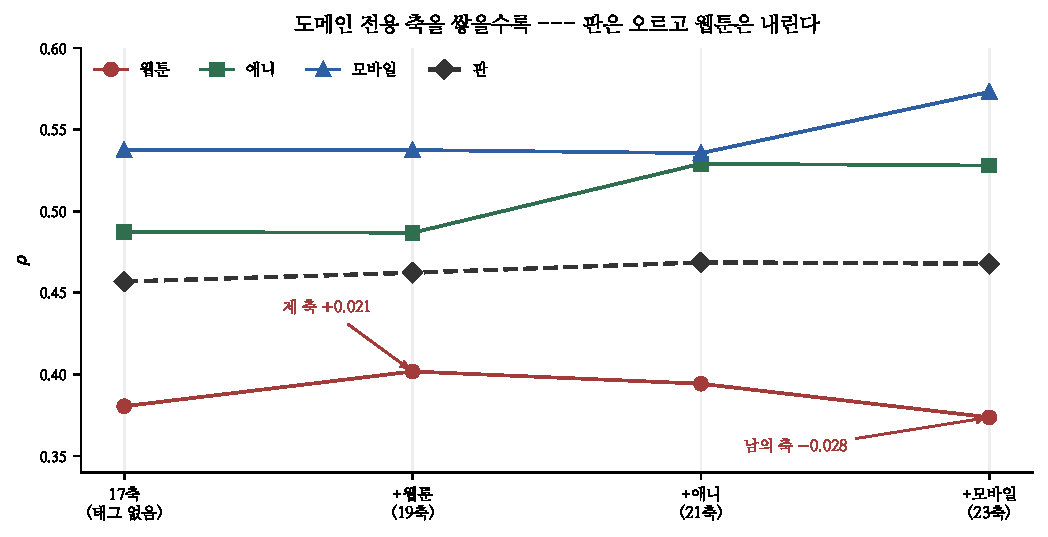
\includegraphics[width=\columnwidth]{figs/crowd.pdf}
\caption{전용 축을 하나씩 쌓으며. 판(검정 점선)은 계속 오르는데 웹툰(빨강)은
제 축에서 한 번 오르고 계속 내린다.}
\end{figure}

\begin{center}\small
\begin{tabular}{lrrrr}
\hline
단계 & 판 & 웹툰 & 애니 & 모바일 \\
\hline
17축 & 0.4569 & 0.3805 & 0.4873 & 0.5374 \\
$+$웹툰 (19축) & 0.4623 & \textbf{0.4018} & 0.4868 & 0.5375 \\
$+$애니 (21축) & 0.4687 & 0.3943 & \textbf{0.5291} & 0.5356 \\
$+$모바일 (23축) & 0.4678 & \textbf{0.3737} & 0.5280 & \textbf{0.5731} \\
\hline
\end{tabular}
\end{center}

\[ \underbrace{+0.0213}_{\text{제 축}} \quad
   \underbrace{-0.0281}_{\text{남의 축}} \quad\Rightarrow\quad
   \text{시작보다 } -0.0068. \]

\textbf{웹툰은 제 축으로 얻은 것보다 남의 축으로 잃은 것이 크다.} 그동안
판은 0.4569에서 0.4687로 올랐다. 판만 보면 축을 놓을 때마다 좋아졌는데,
제일 큰 도메인은 계속 나빠지고 있었다.

\section{가법성이 이전을 덮었다}

노트 250은 ``전용 이름은 가법''이라고 쟀고(교차항/부분합 0.18), 노트 257이
$-$0.0016 으로 다시 확인했다. \textbf{그 말은 판 수준에서만 맞다.}

가법성은 ``각 축이 판에 내는 몫을 따로 더할 수 있다''는 뜻이지 ``각 축이
제 도메인에만 작용한다''는 뜻이 아니다. 웹툰 축은 웹툰만 보고, 애니 축은
애니만 본다 --- 값이 그렇다. 그런데 \textbf{모형은 하나}이고, 열이 늘면
나무의 분할 예산과 능형의 벌점 예산을 나눠 쓴다. 웹툰이 기대던 손 축 다섯의
자리가 좁아진다.

노트 247이 ``판 $\rho$ 는 가중 평균이라 자리바꿈에 눈이 없다''고 적었고,
노트 248이 그것을 SE 로 다듬었다. 이번이 세 번째 얼굴인데 앞의 둘과 다르다
--- \textbf{자리바꿈이 우리가 축을 더할수록 커진다.} 부호화를 바꿀 때(247)나
한 번 재는 것과 달리, 이것은 \emph{누적}이다.

\section{무엇을 할 것인가}

지금 채택한 21축은 그대로 둔다 --- 판 0.4687 이고 웹툰이 시작보다 $+$0.014
위다(0.3805 $\to$ 0.3943). 모바일은 안 넣는다. 넣으면 판은 그대로인데 웹툰이
시작 아래로 떨어진다.

\textbf{규약이 하나 붙는다}: 전용 축을 더할 때 \emph{그 도메인의 이득}만
보지 말고 \textbf{제일 큰 도메인이 얼마 내는지}를 같이 잰다. 몫이 27\%인
도메인이 0.02 내면 판에서 $-$0.006 이라 작은 이득에 묻히는데, 그 도메인
사용자에게는 큰 손해다(노트 254의 판정 단위 대 배포 단위).

\paragraph{남은 것}
\begin{center}\small
\begin{tabular}{ll}
\hline
갈래 & 왜 \\
\hline
자리 예산 & 나무 깊이 · 능형 알파를 축 수에 맞춰 늘리면? \\
웹툰 $t{=}-6.27$ & 제일 뚜렷한 손해. 어느 축을 잃나 \\
게임 259건 & 조각 검사가 못 돈다. 문턱을 안 낮추기로 했다 \\
21축 천장 & 노트 252의 CV 천장을 다시 재야 한다 \\
\hline
\end{tabular}
\end{center}

\paragraph{규약} 전용 축은 공짜가 아니다. \textbf{더할 때마다 제일 큰
도메인의 값을 적는다.} 판이 오르는 것과 모든 도메인이 좋아지는 것은 다른
말이고, 지금 자료에서는 실제로 다르다.

\end{document}
